%%%%%%%%%%%%%%%%%%%%%%%%%%%%%%%%%%%%%%%%%%%%%%%%%%%%%%%%%%%%%%%
%
% Welcome to Overleaf --- just edit your LaTeX on the left,
% and we'll compile it for you on the right. If you open the
% 'Share' menu, you can invite other users to edit at the same
% time. See www.overleaf.com/learn for more info. Enjoy!
%
%%%%%%%%%%%%%%%%%%%%%%%%%%%%%%%%%%%%%%%%%%%%%%%%%%%%%%%%%%%%%%%
\documentclass{beamer}


\hypersetup{
    colorlinks=true,
    linkcolor=blue,
    filecolor=magenta,      
    urlcolor=magenta,
    citecolor=blue!60!black}
\usepackage[english]{babel}
%\usepackage{biblatex}
\usepackage[backend=biber, style=apa]{biblatex}
\addbibresource{references.bib}
\usepackage{booktabs}



%Information to be included in the title page:
\title{A Step Towards Explainable AI: Infer Species Names based on Partial Descriptions}
\author{Robert van de Vlasakker}
\institute{Wageningen University \& Research}
\date{14-12-21}

\begin{document}
\graphicspath{ {./figures/} }

\frame{\titlepage}



% 1 
\begin{frame}
\frametitle{Deep Neural Networks}

Many species will go extinct before ever being described \autocite{lees_species_2015}.
\newline
\newline
Deep Neural Networks can help:
\begin{itemize}
    \item Speed up species identification 
    \item Automate species identification
\end{itemize}


\end{frame}



% 1 
\begin{frame}
\frametitle{Classic Deep Neural Network}
\begin{figure} [htbp]
    \centering
    %\vspace{-2cm}
    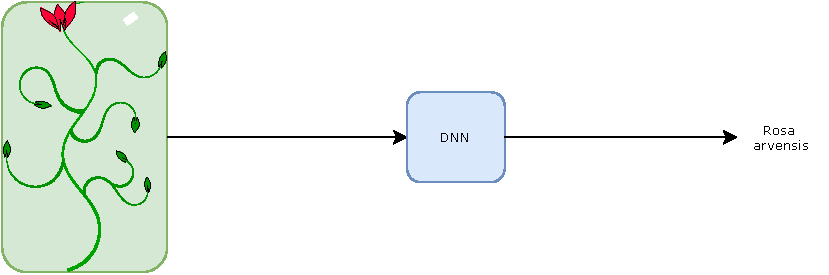
\includegraphics[width=\textwidth]{figures/midterm_explain_1.pdf}
\end{figure}

Takes in an image and makes a prediction.

\end{frame}




% 2 
\begin{frame}
\frametitle{Post Hoc Explanations}
\begin{figure} [htbp]
    \centering
    %\vspace{-2cm}
    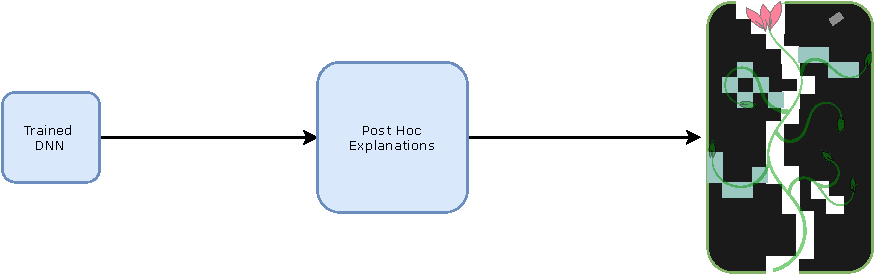
\includegraphics[width=\textwidth]{figures/midterm_explain_2.pdf}
\end{figure}
Post Hoc explanation identify important pixels in the image.
(Black is not important)
\end{frame}


% 3
\begin{frame}
\frametitle{Unidentified Species?}
\begin{figure} [htbp]
    \centering
    %\vspace{-2cm}
    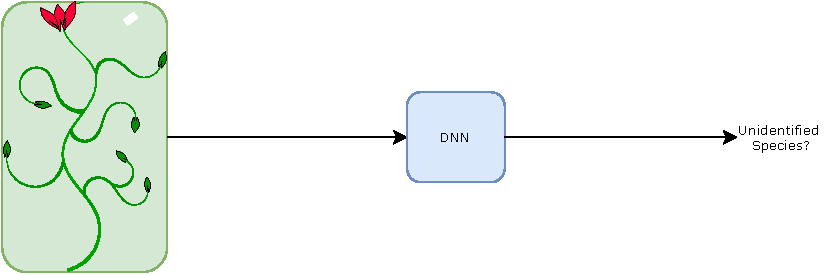
\includegraphics[width=\textwidth]{figures/midterm_explain_3.pdf}
\end{figure}
Post Hoc explanations not very useful:
\begin{itemize}
    \item Difficult to improve models
    \item Difficult to explain models
\end{itemize}
\end{frame}


% 4
\begin{frame}
\frametitle{Proposed Architecture}
\begin{figure} [htbp]
    \centering
    %\vspace{-2cm}
    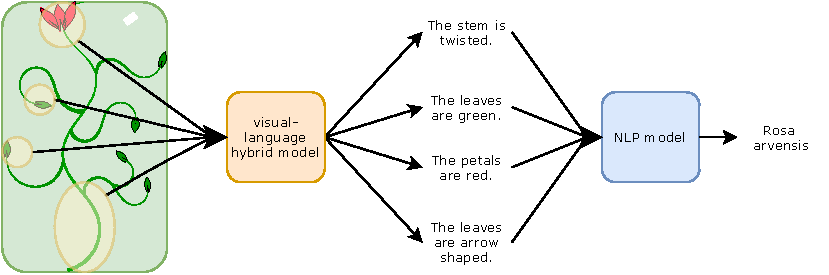
\includegraphics[width=\textwidth]{figures/architecture.pdf}
\end{figure}
Architecture proposal by \textcite{ishikawa_contextual_2021}:
\begin{itemize}
    \item Semantic bottleneck layer
    \item Species can share common traits
\end{itemize}
\end{frame}

% 5
\begin{frame}
\frametitle{Thesis Focus}
\begin{figure} [htbp]
    \centering
    %\vspace{-2cm}
    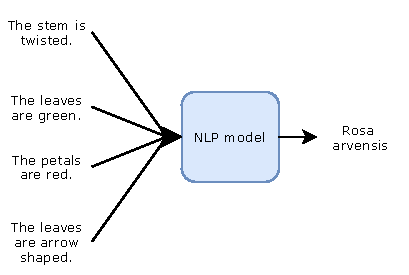
\includegraphics[width=.7\textwidth]{figures/architecture_part.pdf}
\end{figure}
This thesis focus on the NLP model.
Large species database with descriptions is needed.
\end{frame}


% 6
\begin{frame}
\frametitle{Methods}
\begin{figure} [htbp]
    \centering
    %\vspace{-2cm}
    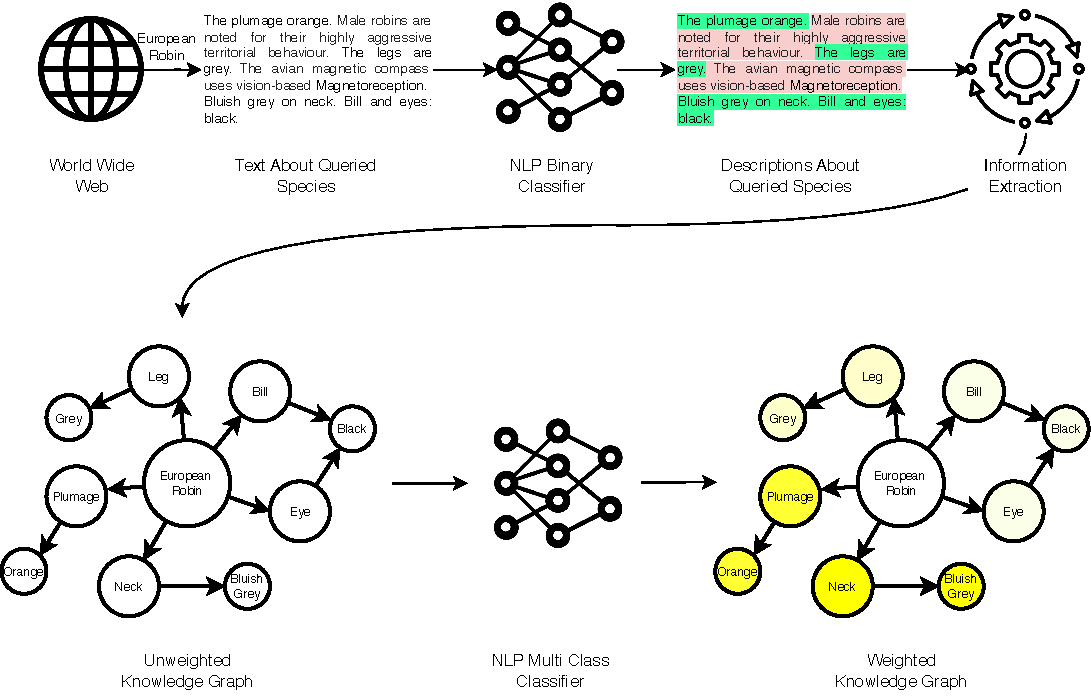
\includegraphics[width=\textwidth]{figures/workflow.pdf}
\end{figure}
\begin{enumerate}
    \item Query species
    \item Check text for descriptions 
    \item Store text that qualify as description
    \item Train NLP model on the data
\end{enumerate}
\end{frame}

% 6
\begin{frame}
\frametitle{Binary Classifier for Descriptions}
\begin{figure} [htbp]
    \centering
    %\vspace{-2cm}
    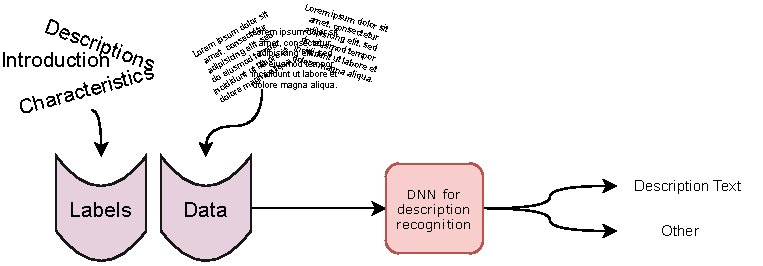
\includegraphics[width=\textwidth]{figures/midterm_explain_4.pdf}
\end{figure}
Data come from several structured sources like Wikipedia:
\begin{itemize}
    \item Text are used a features
    \item Headers are used as labels
\end{itemize}
\end{frame}


% 7
\begin{frame}
\frametitle{Custom Loss Function}
\begin{equation}
 SoftLoss(q, t) = \sum_{k=1}^{L}[\beta t _k + (1- \beta )q _k]log(q _k)
\nonumber\end{equation}
Implement a custom loss function from \textcite{reed_training_2015} to allow semi-supervised learning:
\begin{itemize}
    \item Not all features are correct
    \begin{itemize}
        \item Descriptions can occur in other paragraphs
        \item Non-Descriptions occur in Description paragraphs
    \end{itemize}
    \item If \(\beta\) is reached, the prediction is correct
\end{itemize}
\end{frame}

%8
\begin{frame}
\frametitle{Binary Classification Results}
\begin{figure} [htbp]
    \centering
    %\vspace{-2cm}
    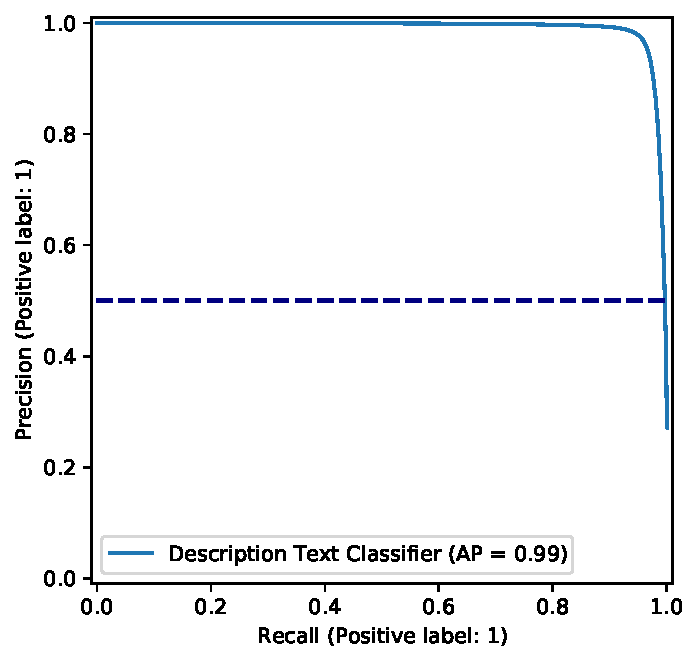
\includegraphics[width=0.45\textwidth]{figures/precision_recall_plot.pdf}
    %\caption{Precision-recall test data}
      \hfill
    %\vspace{-2cm}
    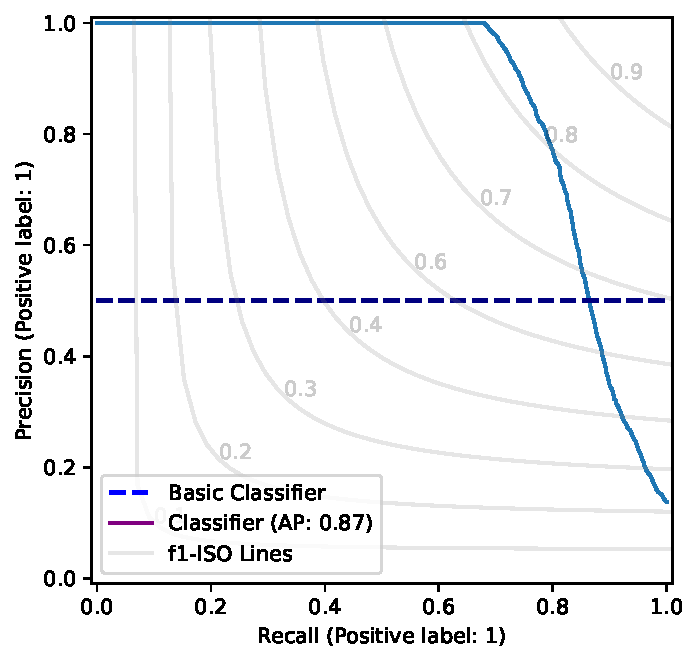
\includegraphics[width=0.45\textwidth]{figures/precision_recall_plot_extern.pdf}
    %\caption{Precision-recall left-out datasets}
\end{figure}
precision-recall plots.

Left: Test dataset

Right: External datasets
\end{frame}

%9
\begin{frame}
\frametitle{Classification Example I}
\begin{figure} [htbp]
    \centering
    %\vspace{-2cm}
    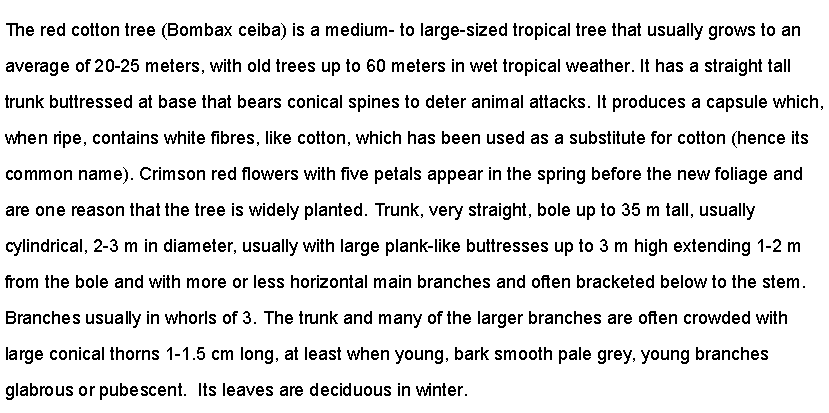
\includegraphics[width=\textwidth]{figures/web_crawler_example_sents_2.pdf}
    %\caption{Source: \href{http://www.llifle.com/Encyclopedia/TREES/Family/Bombacaceae/31994/Bombax_ceiba}{Llilfe.com/Bomax\_ceiba})}
\end{figure}
(Source: \href{http://www.llifle.com/Encyclopedia/TREES/Family/Bombacaceae/31994/Bombax_ceiba}{Llilfe.com/Bomax\_ceiba})
\end{frame}


%10
\begin{frame}
\frametitle{Classification Example II}
\begin{figure} [htbp]
    \centering
    %\vspace{-2cm}
    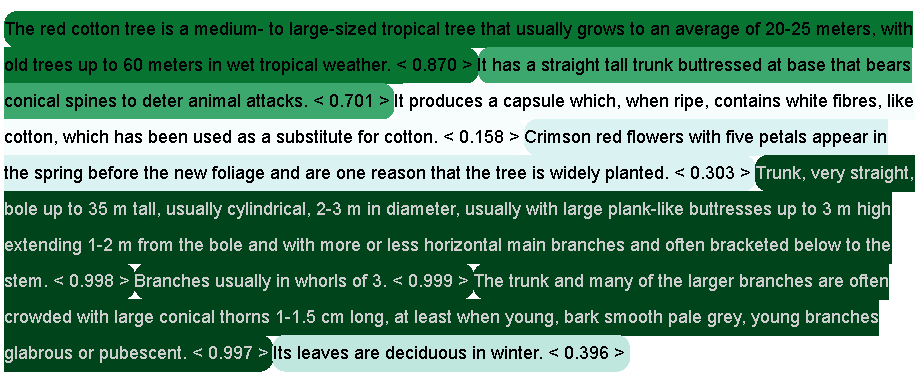
\includegraphics[width=\textwidth]{figures/web_crawler_example_sents_preds_2.pdf}
\end{figure}
\end{frame}



%11
\begin{frame}
\frametitle{And now?}
\begin{itemize}
    \item Web crawler done: iterated over 20,000 species
    \item Descriptions found for ~15,000 species
    \item Train NLP model on the Database
    \item assess NLP model:
    \begin{itemize}
         \item extract most important word combinations? 
         \item present them to a botanist?
         \item How?
    \end{itemize}
\end{itemize}
\end{frame}

%11
\begin{frame}
\frametitle{Assess NLP Model}
\begin{itemize}
    \item Compare with CUB-200 dataset:
    \begin{itemize}
        \item Hand annotated bird dataset
        \item Images with visual traits
    \end{itemize}
    \item Compare posthoc techniques
    \item Train NLP model on own bird descriptions
    \item compute sentence similarity between datasets
\end{itemize}
\end{frame}

%11
\begin{frame}
\frametitle{Similarity Example}
Similarity matrix for one single trait/bird/technique

\begin{figure} [htbp]
    \centering
    %\vspace{0cm}
    %\hspace{-1cm}
    %\textbf{Similarity Matrix}
    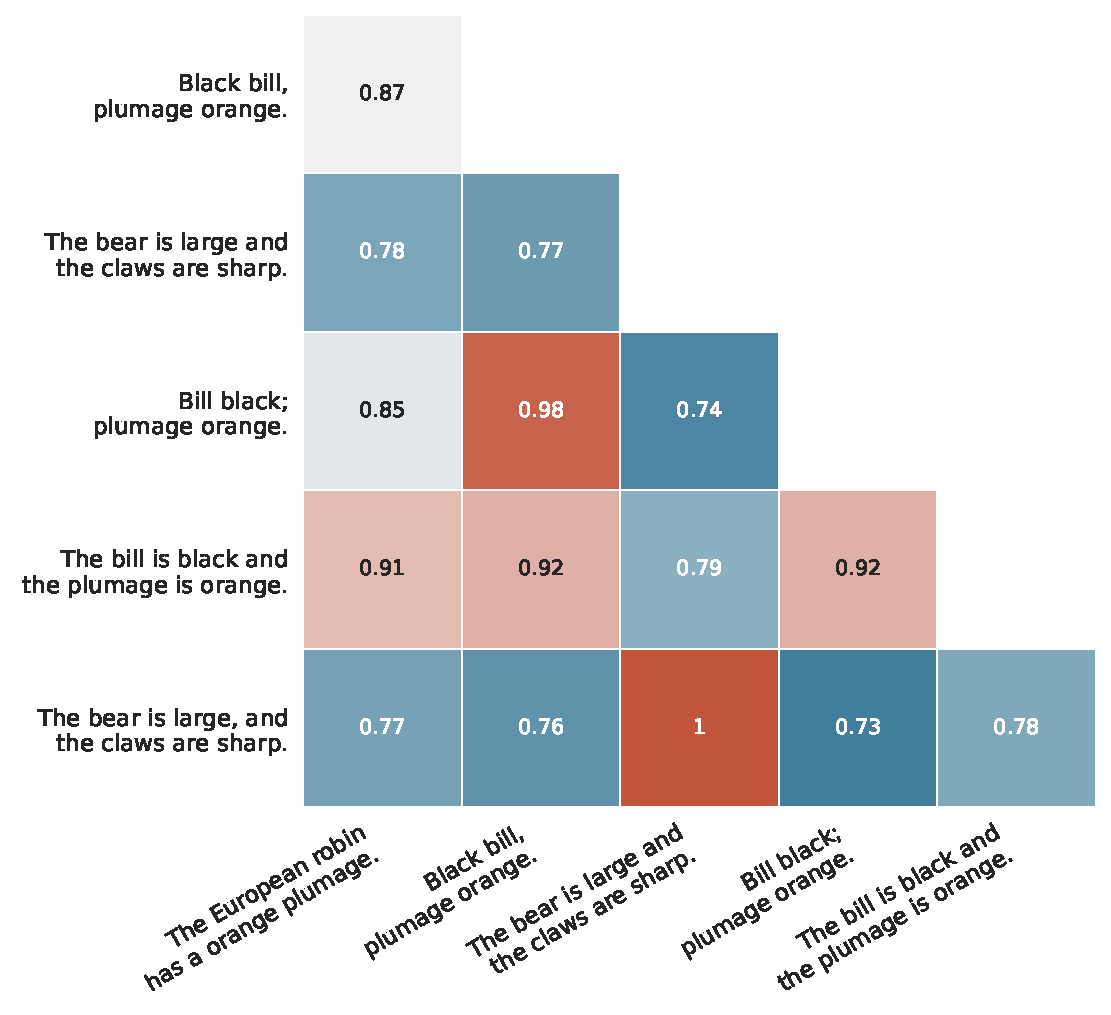
\includegraphics[width=0.7\textwidth]{similarity_matrix.pdf}
\end{figure}

y-axis: CUB-200 data

x-axis: Extracted chunk with posthoc explanation technique
\end{frame}

%12
\begin{frame}
\frametitle{Traits per Country}

\begin{figure}
    \centering
    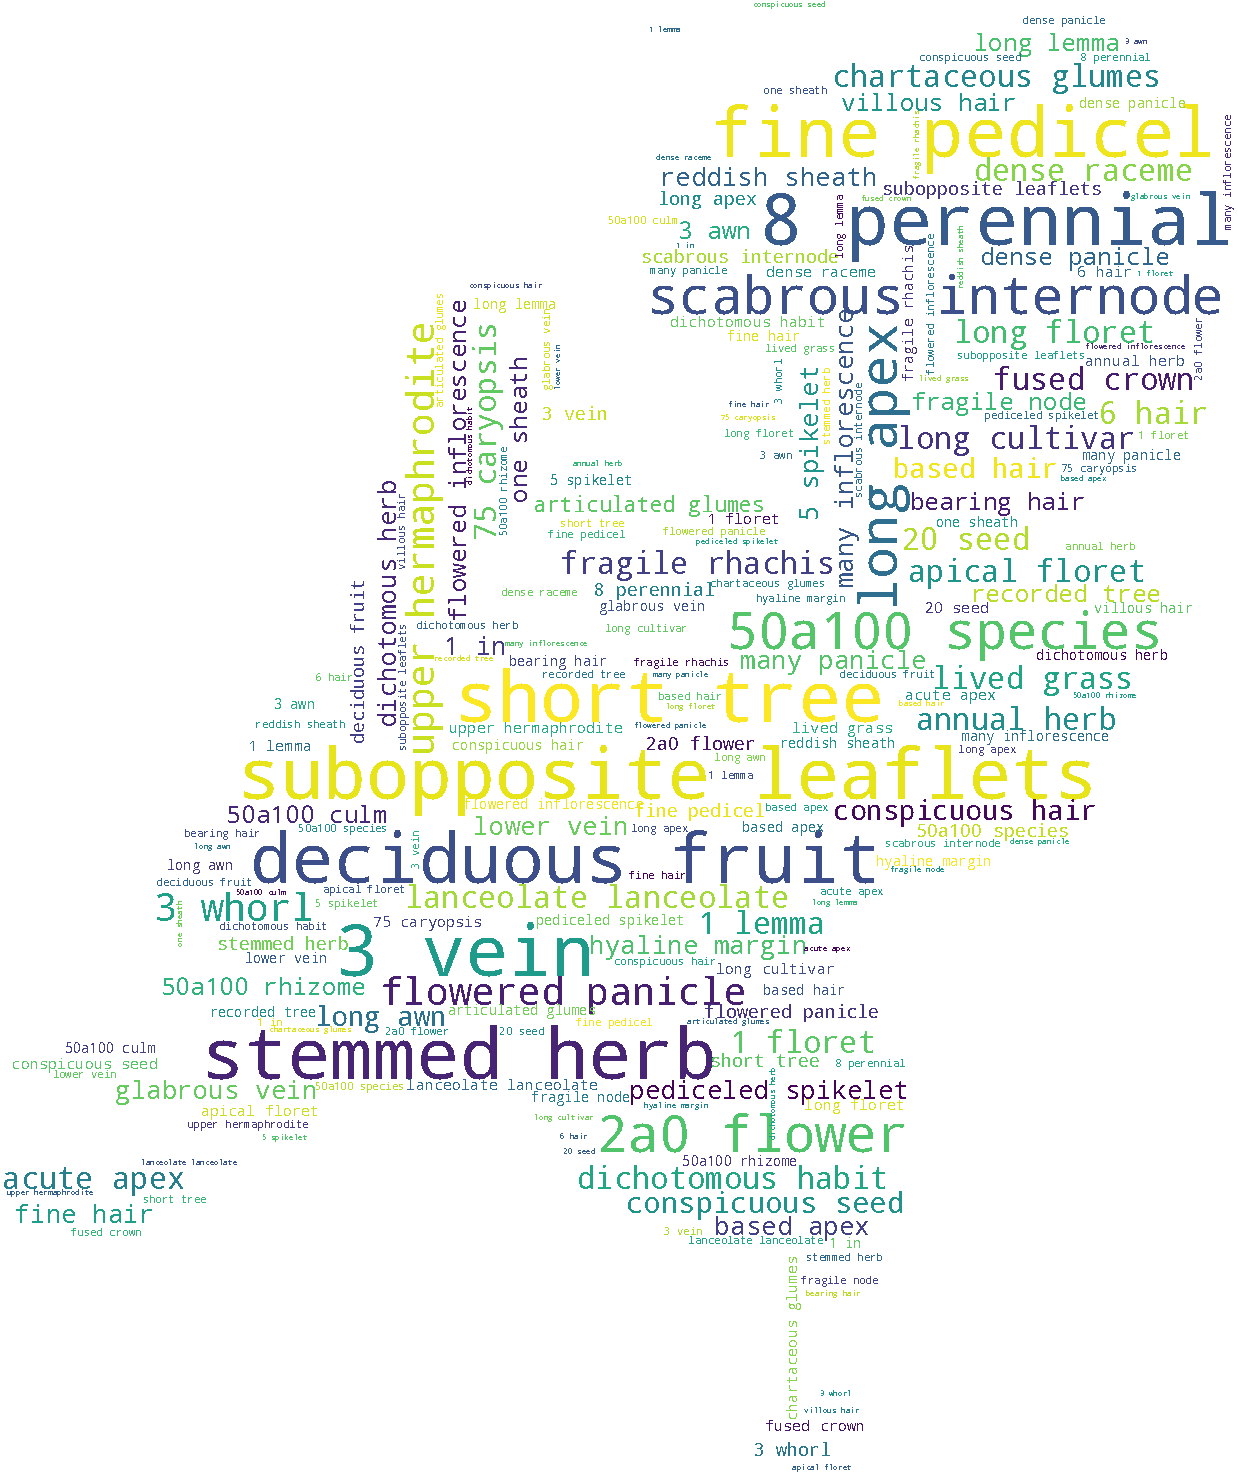
\includegraphics[width=0.7\textwidth]{figures/cover_words.pdf}
\end{figure}

\end{frame}
\end{document}


  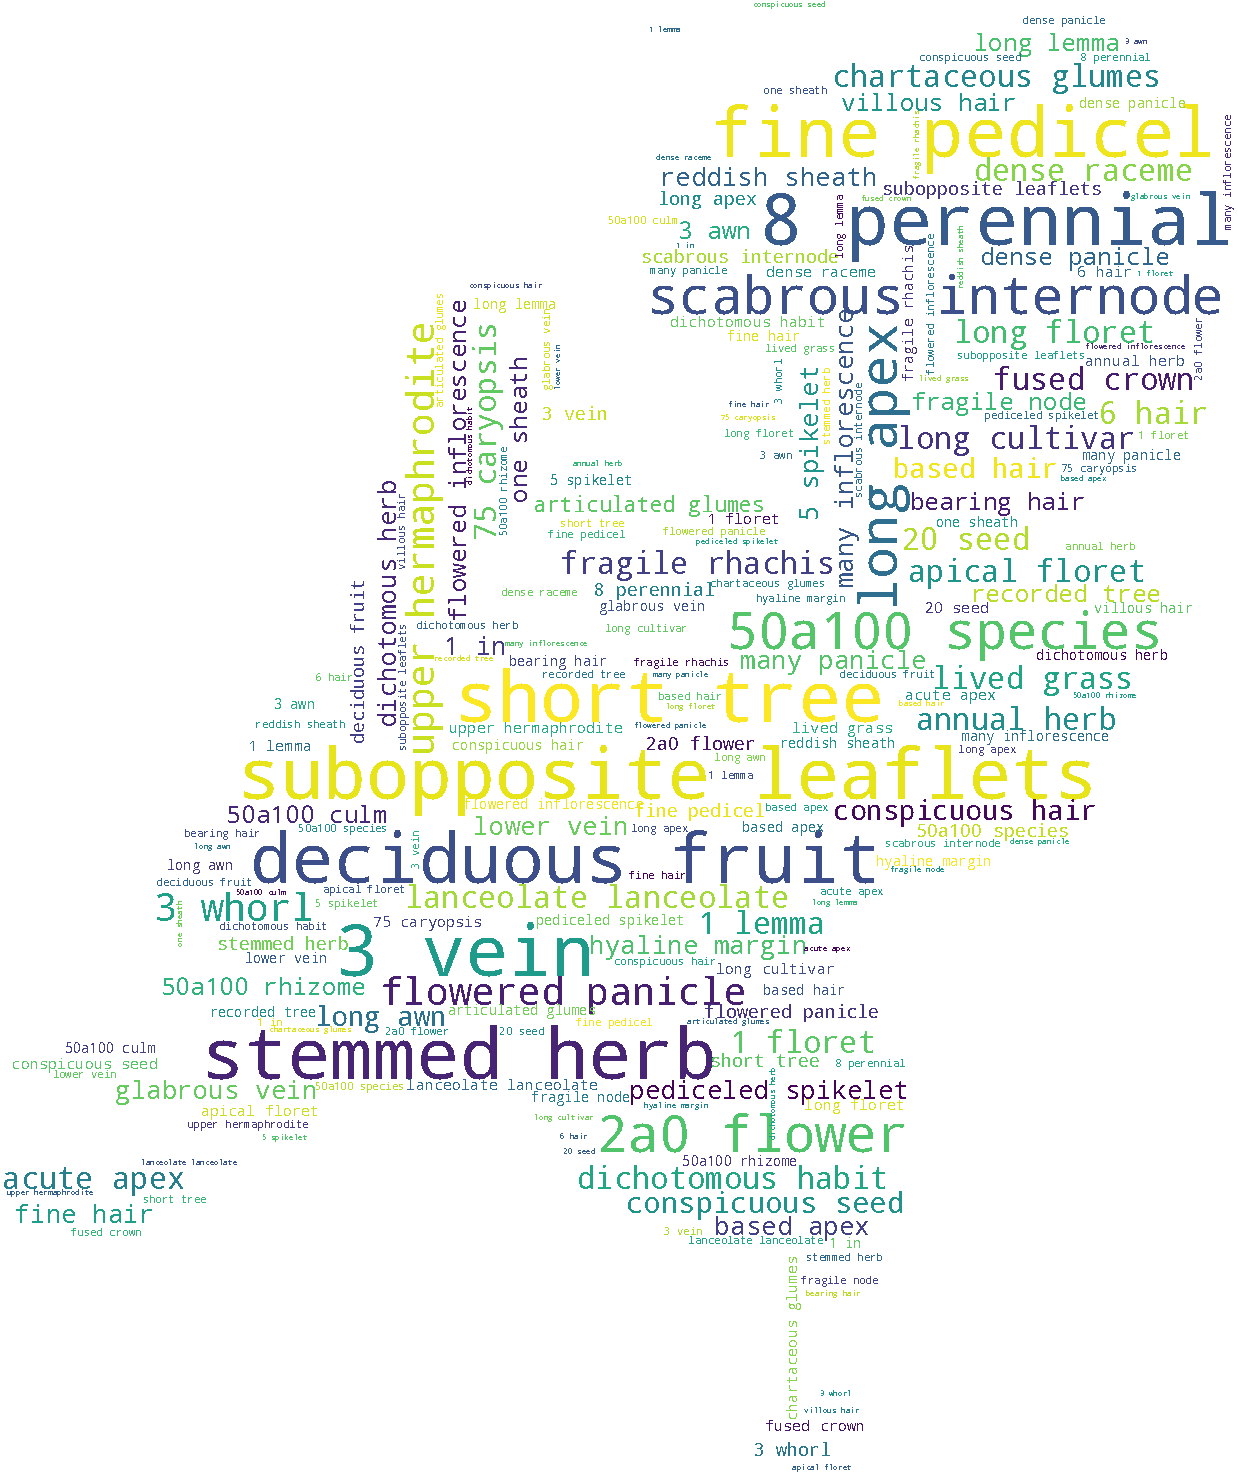
\includegraphics[%
    width=0.85\textwidth,
    %height=0.83\textwidth,
    align=t,
    smash=br,
    vshift=2.5cm,     % adjust the vertical position
    hshift=2.5cm     % adjust the horizontal position
    ]{figures/cover_words.pdf}%